\documentclass[11pt]{article}
%\usepackage{amsfonts}
\usepackage{amsmath}
\usepackage{fancybox}%,times}
\usepackage{graphicx,psfrag,epsf}
%\usepackage{amsmath}
\usepackage{enumerate}
\usepackage{graphicx,psfrag}
\usepackage{multirow}
\usepackage{epsfig}
%\usepackage{rotating}
\usepackage{subfigure}
\usepackage{theorem}
\usepackage{natbib,psfrag}
\usepackage{tikz}
\usepackage{xcolor}
\usepackage{kotex}
\newcommand{\blind}{0}
\usepackage{graphicx}
\DeclareGraphicsExtensions{.pdf,.png,.jpg}

\addtolength{\oddsidemargin}{-.75in}%
\addtolength{\evensidemargin}{-.75in}%
\addtolength{\textwidth}{1.5in}%
\addtolength{\textheight}{1.3in}%
%\addtolength{\topmargin}{-.6in}%
\addtolength{\topmargin}{-.8in}%

%\theoremstyle{break}
\newtheorem{The}{Theorem}
\newtheorem{Def}{Definition}
\newtheorem{Pro}{Proposition}
\newtheorem{Lem}{Lemma}
\newtheorem{Cor}{Corollary}
\newtheorem{asp}{Assumption}


\renewcommand{\thefootnote}{\arabic{footnote}}
%\renewcommand{\thefootnote}{\alph{footnote}}
%\renewcommand{\thefootnote}{\roman{footnote}}
%\renewcommand{\thefootnote}{\fnsymbol{footnote}}

\begin{document}


%\bibliographystyle{natbib}

\newcommand{\Ito}{$It\hat{o}$'$s~Lemma$}

\newcommand\ind{\stackrel{\rm ind}{\sim}}
\newcommand\iid{\stackrel{\rm iid}{\sim}}
\renewcommand\c{\mathbf{c}}
\newcommand\y{\mathbf{y}}
\newcommand\z{\mathbf{z}}
\renewcommand\P{\mathbf{P}}
\newcommand\W{\mathbf{W}}
\newcommand\X{\mathbf{X}}
\newcommand\Y{\mathbf{Y}}
\newcommand\Z{\mathbf{Z}}
\newcommand\J{{\cal J}}
\newcommand\B{{\cal B}}
\newcommand\K{{\cal K}}
\newcommand\N{{\rm N}}
\newcommand\bs{\boldsymbol}
\newcommand\bth{\bs\theta}
\newcommand\bbe{\bs\beta}
\renewcommand\*{^\star}

\def\spacingset#1{\renewcommand{\baselinestretch}%
{#1}\small\normalsize} \spacingset{1}


%%%%%%%%%%%%%%%%%%%%%%%%%%%%%%%%%%%%%%%%%%%%%%%%%%%%%%%%%%%%%%%%%%%%%%%%%%%%%%

  \bigskip
  \bigskip
  \bigskip
  \begin{center}
    {\LARGE\bf Nov 05, 2018 }
  \end{center}
  \medskip

%\begin{abstract}
%\end{abstract}

%\noindent%
%{\it Key Words:}  AECM algorithm; Astrophysical data analysis;
%ECME algorithm; Incompatible Gibbs sampler; Marginal data
%augmentation; Multiple imputation; Spectral analysis

\spacingset{1.45}











\section{Linear Model} 
\subsection{Ordinary Least Square}


  \begin{align}
    \hat{\beta}^{ols} = \min_{\beta} \sum\limits_{i=1}^n (y_{i} - x_{i}^T \beta)^2 
  \end{align}


Ordinary Least Square의 경우 오차의 평균이 0, 오차의 분산이 등분산, 오차가 서로 uncorrelated 일 경우 선형 모형 중에서 최적의 모델이다 (BLUE) 이때 오차의 분포가 정규분포라면 MLE와 동일한 결과를 보여준다

OLS가 아닌 다른 방법을 사용하는 이유는 변수의 개수 p보다 관측치의 개수 n이 충분히 많지 않은 경우 정확한 예측을 하지 못하는 문제가 발생하기 때문이다. 또한 실제 $\beta$값중에서 0이 되어야 하는 $\beta$ 대해서도 0에 가까운 값으로 예측 할 뿐 실제 0으로 예측하지 못하는 문제가 발생한다.

\subsection{Ridge regression}
  \begin{align}
    \hat{\beta}^{ridge} = \min_{\beta} \sum\limits_{i=1}^n (y_{i} - x_{i}^T \beta)^2 + \lambda \sum\limits_{j=1}^p \beta_{j}^2
  \end{align}
L2 regularization term $\lambda \sum\limits_{j=1}^p \beta_{j}^2$ 이 추가되어 있다 기존 OLS와 동일한 부분에서 데이터에 가장 잘 적합하는 동시에 L2 penalty를 통해서 계수들이 0으로 가게 하는 shrink 효과를 부여한다. 이때 L2 regularization term 은 $\beta_{j}$ 가 $X_{j}$의 sclae에 따라 영향을 받는다 따라서 우선적으로 각 변수들을 표준화 해주어야 한다 

least square방법은, unbiased하나 높은 variance를 가진 계수를 추정하게 된다. 이는 데이터가 조금만 바뀌어도 계수들이 크게 변동할 수 있음을 의미한다. 특히, $p>n$, 즉 설명변수가 많아질때 least square는 심지어 유일한 해가 없게 된다. 이러한 상황에서 ridge regression은 약간의 bias에서의 손해로 variance를 크게 줄여 least square보다 좋은 결과를 가져올 수 있다. 쉽게 말해 설명변수$p$ 보다 데이터의 수$n$이 적을때, 더욱 덜 flexible한 적합을 하여 소수의 데이터의 특성에 국한되지 않는 모델을 만드는 것이다.
\subsection{Lasso regression}
  \begin{align}
    \hat{\beta}^{lasso} = \min_{\beta} \sum\limits_{i=1}^n (y_{i} - x_{i}^T \beta)^2 + \lambda \sum\limits_{j=1}^p |\beta_{j}|
  \end{align}
Ridge regression의 단점으로는 중요하지 않은 변수의 $\beta_{j}$를 정확히 0으로 보내지 못한다. Lasso는 적당한 $\lambda$만으로 몇몇 계수를 정확하게 0으로 가게 만들 수 있다. 따라서 몇몇 중요하지 않은 변수가 사라진 효과이므로 해석력에서 ridge보다 강력한 강점을 가지고 있다. 

\section{Nonlinear Model} 
\subsection{Polynomial Regression}

  \begin{align}
	y_{i} = \beta_{0} + \beta_{1}x_{i} + \beta_{2}x_{i}^2  .. \beta_{d}x_{i}^d \\
    \hat{\beta}^{ols} = \min_{\beta} \sum\limits_{i=1}^n (y_{i} - x_{i}^T \beta)^2 
  \end{align}
각 계수들은 OLS를 사용하여서 적합한다. y의 전체 구간에 대해서 non linear형태를 부여한다

\begin{figure}[htbp]
\begin{center}
    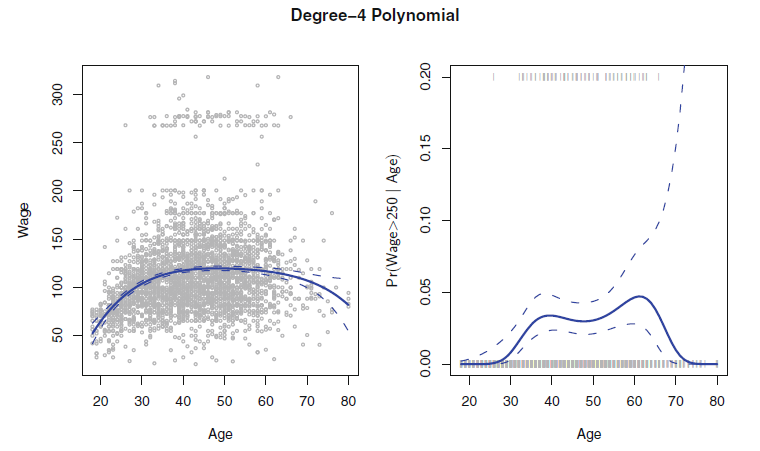
\includegraphics[scale=1.2]{im1}
    \caption{Polynomial Regression} \label{fig:label}
\end{center}
\end{figure}
\subsection{Step Functions}

  \begin{align}
	y_{i} = \beta_{0} + \beta_{1}C_{1}(x_{i}) + \beta_{2}C_{2}(x_{i})  .. \beta_{K}C_{K}(x_{i})  \\
 	\hat{\beta}^{ols} = \min_{\beta} \sum\limits_{i=1}^n (y_{i} - x_{i}^T \beta)^2  \\
	C_{0}(X) = I(X<c_{1}) \\
	C_{1}(X) = I(c_{1} \leq X<c_{1}) \\
	C_{K-1}(X) = I(c_{K-1} \leq X<c_{K}) \\
	C_{K}(X) = I(c_{K} \leq X) 
  \end{align}
전체 X를 K개의 범주로 나누고 각 범주에 대해서 상수를 부여한다. 이 식의 계수들 역시 least square로 적합하여서 구한다
\begin{figure}[htbp]
\begin{center}
    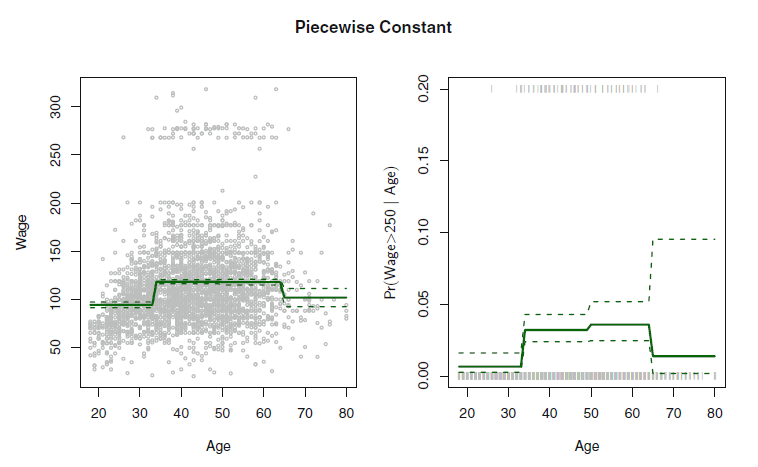
\includegraphics[scale=1.2]{im2}
    \caption{Step Functions} \label{fig:label}
\end{center}
\end{figure}

\subsection{Regression Spines}
전체 X의 범위에 대해서 Polynomial Regression를 적합하는 것이 아니라 구간별로 낮은 차수의 적합을 따로하는 것을 piece wise polynomial regression 이라고 한다 이때 각 범주가 바뀌는 지점을 knots이라고 한다. 이때 knots $\tau$에서 회귀선이 연결되지 않는 문제가 발생한다. 또한 단순히 연결되는 제약조건을 부여할 경우 knots에서 선이 급격하게 꺽여있는 모습을 보인다. 따라서 합리적인 모형을 만들기 위해서 다항식의 차수가 d라고 할때 d-1차 까지의 미분이 가능하게 하여야 한다
  \begin{align}
h(x,\xi) = (x-\xi)^3_{+}\\
y_{i} = \beta_{0} + \beta_{1}X + \beta_{2}X^2 + \beta_{3}X^3   + \beta_{4}h(X,\xi_{1}) + .. + \beta_{K+3} h(X,\xi_{K})
  \end{align}
OLS를 통하여 $\beta$ 값들을 추정하게 된다.
\end{document}
